\documentclass[10pt]{beamer}

\usepackage{../macros}

\usepackage{pgfplots}
\usepgfplotslibrary{dateplot}



\title{La Tortue}

\hypersetup{
  pdftitle =  {La Tortue}
}

\begin{document}

\maketitle

%%%%%%%%%%%%%%%%%%%%%%%%%%%%%%%%%%%%%%%%%%%%%%%%%%%%%%%
\begin{frame}{Les deux types de graphisme dans le plan I}
\subtitle{test}
  Il y a deux types de graphisme 2D, mathématiquement parlant :
  \begin{alertblock}{Le graphisme CARTESIEN (global)}
    Le plan est rapporté à un repère orthonormé direct $(0,\vec{i},\vec{j})$.
  \end{alertblock}

  \begin{block}{Une seule opération essentielle}
    \alert{Tracer un segment} du point $M_1 (x_1,y_1)$ au point $M_2 (x_2, y_2)$.
  \end{block}
  \begin{center}
    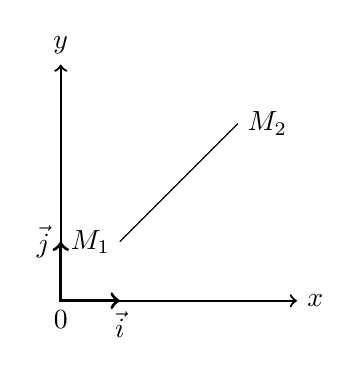
\begin{tikzpicture}[scale=1.5]
      % Draw origin
      \node (0,0) [below] {$0$};
      % Draw axes
      \draw [<->,thick] (0,2) node (yaxis) [above] {$y$}
      |- (2,0) node (xaxis) [right] {$x$};
      % Draw axes
      \draw [<->,very thick] (0,0.5) node (yaxis) [left] {$\vec{j}$}
      |- (0.5,0) node (xaxis) [below] {$\vec{i}$};
      % Draw the segment
      \draw (0.5,0.5) node (M1) [left] {$M_1$} -- (1.5,1.5) node (M2) [right] {$M_2$};
    \end{tikzpicture}
  \end{center}
\end{frame}


%%%%%%%%%%%%%%%%%%%%%%%%%%%%%%%%%%%%%%%%%%%%%%%%%%%%%%%
\begin{frame}{Les deux types de graphisme dans le plan II}

  \begin{alertblock}{Le graphisme POLAIRE (local)}
    Aucune notion de coordonnées.
  \end{alertblock}

  \begin{block}{Deux opérations essentielles :}
    \begin{itemize}
    \item \alert{tourner} à droite ou à gauche sur place d'un angle $a$;
    \item \alert{avancer} dans la direction courante d'une distance $d$
    \end{itemize}
  \end{block}

\begin{columns}[c]
  \begin{column}{0.48\textwidth}
    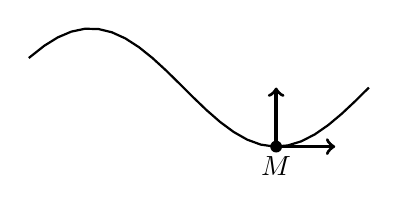
\begin{tikzpicture}[scale=0.75]
    % Draw the curve
    \draw[thick] (pi/6,0.5) -- plot [domain=0.25*pi:2*pi] (\x,{sin(\x r)});
    % Draw the turtle
    \fill (1.5*pi, -1) circle (0.1) node (M) [below] {$M$};
    \draw [->,very thick] (1.5*pi, -1)  -- (1.5*pi+1,-1);
    \draw [->,very thick] (1.5*pi, -1)  -- (1.5*pi,0) ;
  \end{tikzpicture}
  \end{column}
  \begin{column}{0.48\textwidth}
    L'animal traceur porte un repère mobile orthonormé avec une notion de droite et de gauche.
    \\ \alert{la tortue va tourner à gauche}
\end{column}
\end{columns}

\begin{itemize}
\item Opérateurs de translation et de rotation plane, qui engendrent le
groupe des déplacements. La tortue se déplace dans le plan !
\item Graphisme moins matheux, plus intuitif. Inutile de calculer les
coordonnées des points \dots
\item Une trajectoire qui semble lisse sera en fait un polygone !
\end{itemize}
\end{frame}

%%%%%%%%%%%%%%%%%%%%%%%%%%%%%%%%%%%%%%%%%%%%%%%%%%%%%%%
\questionSlide

%%%%%%%%%%%%%%%%%%%%%%%%%%%%%%%%%%%%%%%%%%%%%%%%%%%%%%%
 \appendix
 \backupSlides
%%%%%%%%%%%%%%%%%%%%%%%%%%%%%%%%%%%%%%%%%%%%%%%%%%%%%%%

%%%%%%%%%%%%%%%%%%%%%%%%%%%%%%%%%%%%%%%%%%%%%%%%%%%%%%%
% \begin{frame}[fragile]{Backup slides}
%   Sometimes, it is useful to add slides at the end of your presentation to
%   refer to during audience questions.

%   The best way to do this is to include the \verb|appendixnumberbeamer|
%   package in your preamble and call \verb|\appendix| before your backup slides.

%   will automatically turn off slide numbering and progress bars for
%   slides in the appendix.
% \end{frame}


%%%%%%%%%%%%%%%%%%%%%%%%%%%%%%%%%%%%%%%%%%%%%%%%%%%%%%%
% \begin{frame}[allowframebreaks]{References}

%   % \bibliography{../bib_parallelism,../bib_others}
%   % \bibliographystyle{abbrv}

% \end{frame}

\end{document}

%%% Local Variables:
%%% mode: latex
%%% TeX-master: t
%%% End:
